\chapter{Analytic Solutions to the Neutron Diffusion Equation}
\label{ap:analyticSolutions}

\section{Introduction}
  The following is a manufactured solution designed for verification of one,
  two, and three dimension numerical neutron diffusion equation solvers.
  one group and two group problems are also addressed.
  
  For the reference problems, the one group neutron diffusion problem is written
  below.
  \begin{equation} \label{eq:onegroup}
    -D \grad^2 \phi + \Sigma_r \phi =  \frac{1}{\keff} \nu \Sigma_f \phi + 
      q_{fixed}
  \end{equation}
  For two group neutron diffusion problems, the two group neutron diffusion 
  problem is written below.
  \begin{align} 
    \label{eq:twogroup1}
    -D_1 \grad^2 \phi_1 + \Sigma_{r1} \phi_1 &= \frac{1}{\keff} \left(
      \nu \Sigma_{f1} \phi_1 + \nu \Sigma_{f2} \phi_2 \right) \\
    \label{eq:twogroup2}
    -D_2 \grad^2 \phi_2 + \Sigma_{r2} \phi_2 &= 
      \Sigma_{s 1 \rightarrow 2} \phi_2
  \end{align}
  Where $\phi_1$ is the higher energy group and $\phi_2$ is the lower energy 
  group. This formulation assumes all fission neutrons are created in the fast 
  energy group and there is no up-scattering (scattering that results in an 
  increase in neutron energy). These are realistic assumptions for all diffusive
  neutron systems.

  Analytic solutions are provided herein. One dimension problems can be 
  replicated in a two dimension solver using a square geometry and select 
  boundary conditions. For a given quadrilateral, two of the boundary conditions
  are set to reflective conditions and two are set to zero-flux $(\phi = 0)$ 
  conditions. For true two dimensions problems, all of the boundary conditions 
  are set to zero-flux conditions.
  
  These formula are common to second order partial differential equations but
  the formulation here is based in part from \cite{textbooklewis}.

\section{One Dimension, One Group, Fixed Source}
  \label{sec:deriv_1dfixedsrc}
  This one dimension problem is in the domain $x \in [0,L]$. For this problem, 
  the following one group coefficients are used.
  \begin{align*}
    D &= 1\\
    \Sigma_r &= 1\\
    \nu \Sigma_f &= 0\\
    q_{fixed} &= 1
  \end{align*}
  Then, \eref{eq:onegroup} is written
  \begin{equation} \label{eq:fixed_source}
    - \grad \cdot \grad \phi + \phi = 1 
  \end{equation}
  For notational simplicity, $(\grad \cdot \grad) = \grad^2$. 
  \eref{eq:fixed_source} can also be rewritten.
  \begin{equation} \label{eq:diffusion_simplified}
    \grad^2 \phi - B^2 \phi = S
  \end{equation}
  where $B = 1$ and $S=-1$.
  The solution is composed of a particular and general solution.
  \begin{equation}
    \phi = \phi_g + \phi_p 
  \end{equation}
  For problems of the form of \eref{eq:diffusion_simplified} the general 
  solution has exponential or hyperbolic trigonometric form.
  \begin{equation} \label{eq:fixedsource_general}
    \phi_g = c_1 \cosh(Bx) + c_2 \sinh(Bx)
  \end{equation}
  Where $c_1$ and $c_2$ are problem dependent constants. For $S=1$ as constant
  in the problem domain, the particular solution has given form.
  \begin{align} \label{eq:particular}
    \phi_p &= -S/B \\
           &= 1
  \end{align}
  Then, the combined solution has the given form.
  \begin{equation} 
    \phi = c_1 \cosh(Bx) + c_2 \sinh(Bx) + 1
  \end{equation}
  The only remaining step is to solve for constants $c_1$ and $c_2$. These are
  zero-flux boundary conditions at the problem boundaries.
  \begin{align}
    \label{eq:bcx0}
    \phi(0) &= 0\\
    \label{eq:bcxL}
    \phi(L) &= 0
  \end{align}
  Evaluating the solution at 0, 
  \begin{align}
    \phi(0) &= 0 \\
    &= c_1 + 1\\
    c_1 &= -1
  \end{align}
  Evaluating the solution at $L$
  \begin{align}
    \phi(L) &= 0\\
    &= c_2 \sinh(BL) - \cosh(BL)-1\\
    c_2 &= \frac{\cosh(BL)-1}{\sinh(BL)}
  \end{align}
  The final solution is 
  \begin{equation} \label{eq:analytic_1dfixedsrc}
    \phi(x) = -\cosh(Bx) + \frac{\cosh(BL)-1}{\sinh(BL)} \sinh(Bx) +1
  \end{equation}
  
\section{One Dimension, One Group, Criticality} 
  \label{sec:deriv_1d1g}
  This one dimension problem is in the domain $x \in [0,L]$.
  This problem also uses the one group neutron diffusion equation from 
  \eref{eq:onegroup}. For this problem, and the following coefficients:
  \begin{align*}
    D &= 1\\
    \Sigma_r &= 1\\
    \nu \Sigma_f &= 2\\
    q_{fixed} &= 0
  \end{align*}
  The problem is then proposed as 
  \begin{equation}
    -\grad^2 \phi - \phi = 0 
  \end{equation}
  and has general solution
  \begin{equation} \label{eq:critical_general}
    \phi_g = c_1 \cos(x) + c_2 \sin(x)
  \end{equation}
  Considering zero-flux boundary conditions from \eref{eq:bcx0} and 
  \eref{eq:bcxL}, then $c_1 = 0 $ yielding
  \begin{equation} \label{eq:sinshape}
    \phi_g = c_2 \sin(x)
  \end{equation}
  The problem is an eigenvalue problem and has infinite solutions so the 
  constant $c_2$ is arbitrary for $\sin(x)=0$. Introducing a Buckling term $B$
  then $B=\frac{n \pi}{L}$ and $\sin(Bx)=0$ for $n$ an odd integer. The 
  fundamental mode is then $B=\frac{1}{L}$. Therefore, the solution is 
  \begin{equation} \label{eq:analytic_1d1g}
    \phi = \sin(x/L)
  \end{equation}
  Plugging this solution back into \eref{eq:onegroup} and dividing both sides
  by $\sin(x/L)$ will yield an expression for $\keff$.
  \begin{align}
    -D B^2 + \Sigma_r &= \frac{1}{\keff} \nu \Sigma_f \\
    \keff &= \frac{\nu \Sigma_f}{DB^2 + \Sigma_r} \label{eq:keff1d}
  \end{align}
  Then, for a slab of length $ L = 100 \units{cm} $, $B = \pi / 100$ and
  \begin{equation}
    \keff = 1.9980280254
  \end{equation}
  
\section{Two Dimension, One Group, Criticality}
  \label{sec:deriv_2d1g}
  The same material coefficients are used for this problem as in the 
  one dimension, criticality problem. For this problem, the domain is in the 
  rectangle $[0,L_x]\times[0,L_y]$. Similar to the one-dimension problem, 
  this problem has basic solution of $\sin(x/L)$. The problem is separable in 
  the two spatial dimensions. 
  \begin{equation}
    \phi(x,y) = X(x) Y(y) 
  \end{equation}
  Beginning with equation \eref{eq:onegroup}.
  \begin{align}
    -D \grad^2 \phi(x,y) + \Sigma_r \phi(x,y) &= \nu \Sigma_f \phi(x,y) \\
    - \grad^2 \phi(x,y) - \phi(x,y) &= 0 \\
    \grad^2 \phi(x,y) + \phi(x,y) &= 0 \\
    \frac{\partial^2}{\partial x^2} \phi(x,y) + 
      \frac{\partial^2}{\partial y^2} \phi(x,y) +
      \phi(x,y) &= 0\\
    Y(y)\frac{\partial^2}{\partial x^2}X(x) +
      X(x) \frac{\partial^2}{\partial y^2} Y(y) + X(x)Y(y) &= 0\\
    Y(y)\left(\frac{\partial^2}{\partial x^2}X(x) + \frac{1}{2} X(x)\right)+
      X(x)\left(\frac{\partial^2}{\partial y^2}Y(y) + \frac{1}{2}Y(y)
      \right) &= 0
  \end{align}
  For non-trivial solutions $X(x) \ne 0$ and $Y(y) \ne 0$ then the following
  second order ordinary differential equations can be solved.
  \begin{align}
    \frac{d^2}{dx^2} X(x) + \frac{1}{2} X(x) &= 0 \\
    \frac{d^2}{dy^2} Y(y) + \frac{1}{2} Y(y) &= 0 \\
  \end{align}
  The solution to these problems is the product of the solutions from the 
  previous problem presented in \eref{eq:analytic_1d1g}. The solution is
  \begin{equation} \label{eq:analytic_2d1g}
    \phi(x,y) = \sin(x/A) \sin(y/B)
  \end{equation}
  Where $L_x$ is the horizontal extent of the rectangular domain and $L_y$ is 
  the vertical extent of the rectangular domain. Extending the concept of 
  geometric buckling to the two spatial dimensions where $B_x = \frac{1}{L_x}$
  and $B_y = \frac{1}{L_y}$. If $B=B_x=B_y$; that is, $L_x=L_y$, $\keff$ can 
  be calculated as
  \begin{equation}
    \keff = \frac{\nu \Sigma_f}{2DB^2 + \Sigma_r} 
  \end{equation}
  Then, for $A=B = 100 \units{cm}$
  \begin{equation}
    \keff = 1.9960599356
  \end{equation}
  
\section{One Dimension, Two Group, Criticality}
  \label{sec:deriv_1d2g}
  Much of this section is drawn from course notes prepared by Dr. Scott 
  Palmtag \cite{analytic2g}.
  
  A two group neutron diffusion problem is considered for a one-dimension
  homogeneous slab in the domain $x \in [0,L]$. Energy group 1 is higher energy
  than energy group 2. It is assumed all fission neutrons are  produced in the
  fast group (i.e. $\chi_1=1$ and $\chi_2=0$). Additionally, it is assumed that 
  there is no up-scattering  (i.e. $\Sigma_{2\rightarrow1}=0$).  Then, the
  two group neutron diffusion equations are given in \eref{eq:twogroup1} and 
  \eref{eq:twogroup2}.
  
  Referring to the problem posed by Section \sref{sec:deriv_1d1g}, the flux 
  solutions have form given in equation \eref{eq:sinshape}. Then
  \begin{align}
    \label{eq:twogroupflux1}
    \phi_1 &= c_1 \sin(Bx) \\
    \label{eq:twogroupflux2}
    \phi_2 &= c_2 \sin(Bx)
  \end{align}
  Where $B$ is the geometric buckling term. For this geometry, the geometric 
  buckling of the fundamental mode is given by 
  \begin{equation}
    B = \pi/L
  \end{equation}
  Then, plugging  \eref{eq:twogroupflux1} and \eref{eq:twogroupflux2} into 
  \eref{eq:twogroup2} and dividing the equation by $\sin(Bx)$
  \begin{equation}
    D_2 B^2 c_2 + \Sigma_{r2} c_2 = \Sigma{s1\rightarrow2} c_1
  \end{equation}
  Then, the ratio can be expressed
  \begin{equation} \label{eq:fluxratio}
    \frac{c_2}{c_1} = \frac{\Sigma_{s1\rightarrow2}}{D_2 B^2 + \Sigma_{r2}}
  \end{equation}
  The ratio $\frac{c_2}{c_1}$ represents the relative magnitude of thermal to 
  fast flux. Returning to \eref{eq:twogroup1}, pluggin in 
  \eref{eq:twogroupflux1} and \eref{eq:twogroupflux2} and again dividing both
  sides by  $\sin(Bx)$
  \begin{align}
    D_1 B^2 c_1 &= \frac{1}{\keff} \left( \nu \Sigma_{f1} c_1 + 
      \nu \Sigma_{f2} c_2\right)\\
    \keff &= \frac{\nu \Sigma_{f1} c_1 + \nu \Sigma_{f2} c_2}
      {D_1 B^2 c_1 + \Sigma{r1} c_1}\\
    \keff &= \frac{\nu \Sigma_{f1} + \nu \Sigma_{f2} c_2/c_1}
      {D_1 B^2 + \Sigma{r1}}
  \end{align}
  Plugging in the expression from \eref{eq:fluxratio}
  \begin{equation}
    \keff = \frac{\nu \Sigma_{f1} + \nu \Sigma_{f2} 
      \left(\frac{\Sigma_{s1\rightarrow2}}{D_2B^2+\Sigma_{r2}}\right)}
      {D_1 B^2 + \Sigma{r1}}
  \end{equation}
  From the VVER-440 benchmark, material 1,
  \begin{align*}
    D_1 &= 1.3466  \\
    D_2 &= 0.37169 \\
    \Sigma_{r1} &= 2.5255\text{E}-2\\
    \Sigma_{r2} &= 6.4277\text{E}-2\\
    \nu \Sigma_{f1}  &= 4.4488\text{E}-3\\
    \nu \Sigma_{f2}  &= 7.3753\text{E}-2\\
    \Sigma_{s1\rightarrow2} &= 1.6893\text{E}-2 \\
    k_{\infty} &= 0.943664259
  \end{align*}
  For a 100 \units{cm} slab.
  \begin{align}
    \frac{c_2}{c_1} &= 0.26132419 \\
    \keff &= 0.892349025
  \end{align}
  
\section{One Dimension, One Group, Two Region, Criticality}
  \label{sec:deriv_2reg}
  This final analytic problem was designed to test the materials mapping of a
  solver. The problem is proposed as a slab-reactor with a fuel and  reflector
  region. The neutron diffusion equation is given in  \eref{eq:onegroup}. 
  Geometry is described in \fref{fig:2reg_geom}. Fuel Material (subscript F) 
  is located in $x \in [0,a]$ and Reflector Material (subscript R) is located in
  $x \in [a,b]$.
  \begin{figure}
    \centering
    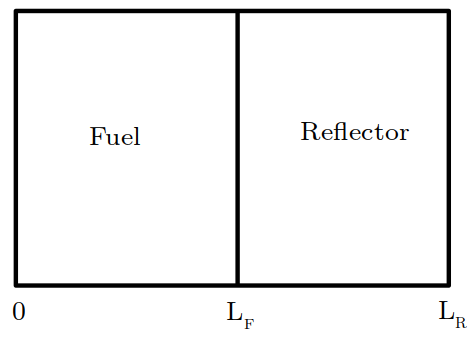
\includegraphics[width=0.6\textwidth]{2reg_geom}
    \caption{Geometry for Two Region Problem.}
    \label{fig:2reg_geom}
  \end{figure}
  Boundary conditions on the horizontal surfaces (top/bottom) are reflective
  to reduce the problem to one-dimension. Other boundary conditions are given
  below. Noting $\phi'(x) = \frac{d \phi}{dx}$.
  \begin{align}
    \label{eq:2reg_mirror}
    \phi'_F(0)&=0\\
    \label{eq:2reg_continuity}
    D_F\phi'_F(a)&=D_R\phi'_R(a) \\
    \label{eq:2reg_fluxcontinuity}
    \phi_F(a) &= \phi_R(a) \\
    \label{eq:2reg_zeroflux}
    \phi_R(b)&=0
  \end{align}
  These represent mirror condition at $x=0$, current continuity at $x=a$, flux
  continuity at $x=a$, and zero-flux at $x=b$. The material properties are 
  specified in \tref{tab:2reg_constants}.
  \begin{table}
    \caption{Two Region Material Constants.}
    \label{tab:2reg_constants}
    \begin{center}
      \begin{tabular}{crr}
        \toprule
        & Fuel & Reflector \\
        \midrule
        $D$ & 1.2 & 0.7 \\
        $\Sigma_r$ & 0.02 & 0.015 \\
        $\nu \Sigma_f$ & 0.02 & 0 \\
        $q_{fixed}$ & 0 & 0 \\
        \bottomrule
      \end{tabular}
    \end{center}
  \end{table}
  
  The general form of the solution in the fueled region has form similar to 
  \eref{eq:critical_general}.
  \begin{equation}
    \phi_F(x) = c_{1F} \cos(B_F x) + c_{2F} \sin(B_F x)
  \end{equation}
  Then, using the mirror boundary condition at $x=0$ \eref{eq:2reg_mirror}.
  \begin{align}
    \phi_F(x) &= c_{1F} \cos(B_F x) + c_{2F} \sin(B_F x) \\
    \phi'_F(x) &= -B_F c_{1F} \sin(B_F x) + B_F c_{2F} \cos(B_F x) \\
    \phi'_F(0) &= 0\\
    &=B_F c_{2F}
  \end{align}
  Therefore, $c_{2F}=0$ and
  \begin{equation}
    \phi_F(x) = c_{1F} \cos(B_F x)
  \end{equation}
  Because this is an eigenvalue problem, $c_{1F}$ is arbitrary and $B_F$ 
  represents the buckling factor in the Fuel Material.
  
  Now for the solution in the reflector region. The solution has general form
  similar to \eref{eq:fixedsource_general}.
  \begin{equation}
    \phi_R(x) = c_{1R} \cosh(B_R (x-a)) + c_{2R} \sinh(B_R (x-a))
  \end{equation}
  The coordinate transform $(x-a)$ is equivalent to multiplying by a constant 
  because $\sinh$ and $\cosh$ can be rewritten as exponentials and due to 
  exponential properties. Treating the zero-flux boundary condition at $x=b$ 
  \eref{eq:2reg_zeroflux}.
  \begin{align}
    \phi_R(x) &= c_{1R} \cosh(B_R (x-a)) + c_{2R} \sinh(B_R (x-a))\\
    \phi_R(b) &= 0 \\
    &= c_{1R} \cosh(B_R(b-a)) + c_{2R} \sinh(B_R(b-a))\\
    c_{1R} &= -c_{2R} \frac{\sinh(B_R(b-a))}{\cosh(B_R(b-a))}\\
    c_{1R} &= -c_{2R} \tanh(B_R(b-a))\\
    c_{2R} &= -c_{1R} \frac{1}{\tanh(B_R(b-a))} \label{eq:c2rnumber1}
  \end{align}
  Treating the current continuity boundary condition at $x=a$ 
  \eref{eq:2reg_continuity}.
  \begin{align}
    D_F \phi'_F(a) &= D_R \phi'_R(a) \\
    -D_F c_{1F} B_F \sin(B_F a) &= D_R B_R c_{2R} \\
    c_{2R} &= -\frac{D_F c_{1F} B_F \sin(B_F a)}{D_R B_R} \label{eq:c2rnumber2}
  \end{align}
  Treating the flux continuity boundary condition at $x=a$ 
  \eref{eq:2reg_fluxcontinuity}.
  \begin{align}
    \phi_F(a)&=\phi_R(a) \\
    c_{1F} \cos(B_F a) &= c_{1R} \\
    c_{1R} &= c_{1F} \cos(B_F a) \label{eq:c1r}
  \end{align}
  Setting equations \eref{eq:c2rnumber1} and \eref{eq:c2rnumber2} equal.
  \begin{equation}
    - \frac{D_F c_{1F} B_F \sin(B_F a)}{D_R B_R} = -c_{1R} \tanh(B_R(b-a))
  \end{equation}
  Plugging in the the expression for $c_{1R}$ from \eref{eq:c1r}
  \begin{align}
    - \frac{D_F c_{1F} B_F \sin(B_F a)}{D_R B_R} &=
      - \frac{c_{1F} \cos(B_F a)}{\tanh(B_R(b-a))}\\
    \frac{D_F B_F \sin(B_F a)}{D_R B_R} &= 
      \frac{\cos(B_F a)}{\tanh(B_R(b-a))} \\
    B_F \tan(B_F a) &= \frac{D_R B_R}{D_F \tanh(B_R(b-a))}
  \end{align}
  By material definition,  ${B_R = \sqrt{\Sigma_{rR}/D_R}}$.
  
  This is the most simplified solution. Unfortunately, there is no analytic
  expression for $B_F$. Therefore, a numeric solver must be used such as 
  MATLAB's \texttt{vpasolve()} or a generic bisection/binary search. The $\tan()$ 
  function causes the solution to $B_F$ is especially sensitive to the starting
  guess.
  
  Once $B_F$ is known, the problem is solved.
  \begin{align}
    \phi_F(x) &= \phi_0 \cos(B_F x)\\
    \phi_R(x) &= \phi_0 \cos(B_F a) \cosh(B_R (x-a)) 
      - \frac{D_F \phi_0 \sin(B_F a)}{D_R B_R} \sinh(B_R (x-a))\\
    \label{eq:analytic_2reg}
    \phi(x) &= H(x-a)\phi_R(x) + H(a-x)\phi_F(x)
  \end{align}
  Where $H(x)$ is the Heaviside step function.  
  
  The eigenvalue for this problem can be expressed for a known $B_F$. Similar 
  to \eref{eq:keff1d}. In this problem, for $a=50 \units{cm}$ and
  $b=100 \units{cm}$ and material constants given in \tref{tab:2reg_constants}.
  \begin{align}
    B_F &= 0.0255922048213879 \\
    \keff &= \frac{\nu\Sigma_{fF}}{D_F B_F^2 + \Sigma_{rF}} \\
    &= 0.9621882561
  \end{align}
  
\section{Finite Cylinder, One Group, Criticality}
  \label{sec:deriv_finite_cyl}
  The finite cylinder is an example of a truly three-dimension problem with
  an analytic solution. This is a homogeneous cylinder with zero-flux boundary
  conditions on the edge of the cylinder. The cylinder has height $H$ and 
  radius $T$. The coordinates $r\in[0,T]$ and $z\in[0,H]$ where 
  $r=\sqrt{x^2+y^2}$.
  
  The solution method is by separation of variables into radial and axial 
  directions. This derivation is similar to that in \sref{sec:deriv_2d1g}.
  Beginning with the one group neutron diffusion equation \eref{eq:onegroup} and assuming
  that  $\phi(r,z) = R(r) Z(z)$.
  \begin{align}
    -D \grad^2 \phi(r,z) + \Sigma_r \phi(r,z) &= \nu \Sigma_f \phi(r,z) \\
    \grad^2 \phi(r,z) + \frac{\nu\Sigma_f - \Sigma_r}{D} \phi(r,g) &= 0 \\
    \frac{1}{r} \frac{\partial}{\partial r} \left( r \frac{\partial}{\partial r}
      \phi(r,z) \right) + \frac{\partial^2}{\partial z^2} \phi(r,z) +
      \frac{\nu\Sigma_f - \Sigma_r}{D} \phi(r,z) &= 0 \\
    Z(z) \frac{1}{r} \frac{\partial}{\partial r} \left( r 
      \frac{\partial}{\partial r} R(r) \right) + 
      R(r) \frac{\partial^2}{\partial z^2} Z(z) + 
      \frac{\nu\Sigma_f - \Sigma_r}{D} R(r) Z(z) &= 0 \\
    Z(z) \frac{1}{r} \frac{\partial}{\partial r} \left( r 
      \frac{\partial}{\partial r} R(r) \right) + 
      R(r) \frac{\partial^2}{\partial z^2} Z(z) + 
      B^2 R(r) Z(z) &= 0 \\
    Z(z) \left( \frac{1}{r} \frac{\partial}{\partial r} \left( r 
      \frac{\partial}{\partial r} R(r) \right) + \frac{B^2}{2} R(r) \right) + 
      R(r) \left( \frac{\partial^2}{\partial z^2} Z(z) + \frac{B^2}{2} Z(z) 
      \right) &= 0
  \end{align}
  For non-trivial solutions $R(r) \ne 0$ and $Z(z) \ne 0$ then the following
  second order ordinary differential equations can be solved.
  \begin{align}
    \label{eq:cyl_radialR}
    \frac{1}{r} \frac{\partial}{\partial r} \left( r \frac{\partial}{\partial r}
      R(r) \right) + \frac{B^2}{2} R(r) &= 0 \\
    \label{eq:cyl_axialZ}
    \frac{\partial^2}{\partial z^2} Z(z) + \frac{B^2}{2} Z(z) &= 0
  \end{align}
  
  Beginning with the axial direction. The diffusion equation can be rewritten as 
  \eref{eq:cyl_axialZ}.
  \begin{equation} \label{eq:simplediffusion}
    \grad^2 Z(z) + B_z^2 Z(z) = 0
  \end{equation}
  and has solution of the form \eref{eq:critical_general}.
  \begin{equation} \label{eq:cyl_axial}
    Z(z) = c_1 \cos(B_z z) + c_2 \sin(B_z z)
  \end{equation}
  Requiring zero-flux boundary conditions $\phi(0)=\phi(H)=0$ yields $c_1=0$. 
  Then $c_2$ is arbitrary and the buckling condition is $B_zH=\pi$ and $B_z=\pi/H$.
  
  Moving on to the radial direction. The diffusion equation can be written as
  \eref{eq:cyl_radialR}.
  \begin{equation}
    \grad^2 R(r) + B_r^2 R(r) = 0
  \end{equation}
  Noting the radial coordinates.
  \begin{align}
    \frac{1}{r} \frac{\partial}{\partial r} \left( r \frac{\partial R}
      {\partial r} \right) + B_r^2 R &= 0 \\
    \frac{\partial}{\partial r} \left( r \frac{\partial R}{\partial r}
      \right) + B_r^2 R &= 0
  \end{align}
  Noting the product rule of differentiation.
  \begin{align}
    r \frac{\partial^2 R}{\partial r^2} + \frac{\partial R}
      {\partial r} + B_r^2 r R &= 0 \\
    \frac{\partial^2 \phi}{\partial r^2} + \frac{1}{r} \frac{\partial R}
      {\partial r} + B_r^2 R &= 0 \label{eq:besselequation}
  \end{align}
  Noting equation \eref{eq:besselequation}, \cite{textbooklewis} Appendix B
  shows the equation has solution of the form
  \begin{equation} \label{eq:cyl_radial}
    R(r) = c_3 J_0(B_r r) + c_4 Y_0(B_r r)
  \end{equation}
  Where $J_0$ is the Bessel function of the first kind, zeroth order and $Y_0$
  is the Bessel function of the second kind, zeroth order. Requiring the flux
  to be finite at $r=0$ requires $c_4=0$ as 
  $\lim_{r\rightarrow0} Y_0(r) \rightarrow -\infty$. As this is an eigenvalue
  problem, $c_3$ is arbitrary. Zero flux boundary conditions requires 
  $B_r R=\alpha_0$ where $\alpha_0$ is the first root of the $J_0$ function and 
  $\alpha_0 \approx 2.4048$. Then $B_r=\alpha_0/R$.
  
  Combining the radial expression \eref{eq:cyl_radial} and the axial 
  expression \eref{eq:cyl_axial} yields the final expression for the flux.
  \begin{align} \label{eq:analytic_finite_cyl}
    \phi(r,z) &= J_0(B_r r) \sin(B_z z) \\
    &= J_0(r \alpha_0 / R) \sin(z \pi / H)
  \end{align}
  Plugging \eref{eq:analytic_finite_cyl} into the diffusion equation will yield the 
  buckling/criticality condition.
  \begin{equation}
    -D \left( \frac{1}{r} \frac{\partial}{\partial r} \left( r 
      \frac{\partial \phi}{\partial r} \right) + \frac{\partial^2 \phi}
      {\partial z^2} \right) + \Sigma_r \phi = \frac{1}{\keff} \nu 
      \Sigma_f \phi
  \end{equation}
  Beginning with the differentiation terms for simplicity. Axial 
  differentiation is straight-forward and presented below.
  \begin{equation}
    \label{eq:above}
    \frac{\partial^2 \phi}{\partial z^2} = -B_z^2 J_0(B_r r) \sin(B_z z)
  \end{equation}
  Radial differentiation must account for the radial geometry and is more 
  complex. First, note the following derivative relationship of the zeroth
  order Bessel function.
  \begin{equation} \label{eq:deriv_bessel0}
    \frac{d}{dr} J_0(\alpha r) = - \alpha J_1(\alpha r)
  \end{equation}
  And applying \eref{eq:deriv_bessel0} to \eref{eq:above}
  \begin{align}
    \frac{\partial \phi}{\partial r} &= -B_r \sin(B_z z) J_1(B_r r) \\
    r \frac{\partial \phi}{\partial r} &= -B_r \sin(B_z z) r J_1 (B_r r) 
  \end{align}
  Note the additional derivative relation for the general Bessel function.
  \begin{equation} \label{eq:deriv_besseln}
    \frac{d}{dr} J_n(r) = \frac{1}{2} \left( J_{n-1}(r) - J_{n+1}(r)\right)
  \end{equation}
  Evaluating the rest of the cylindrical derivative using
  \eref{eq:deriv_besseln} and the product rule.
  \begin{align}
    \frac{\partial}{\partial r} \left( r \frac{\partial \phi}{\partial r}
      \right) &= -B_r \sin(B_z z) \left(J_1(B_r r) + \frac{1}{2} B_r r \left(
      J_0(B_r r) - J_2(B_r r) \right) \right) \\
    \frac{1}{r} \frac{\partial}{\partial r} \left(r 
      \frac{\partial \phi}{\partial r} \right) &=
      -B_r \sin(B_z z) \left(\frac{1}{r} J_1(B_r r) + \frac{1}{2} B_r \left(
      J_0(B_r r) - J_2(B_r r) \right) \right)
  \end{align}
  Finally, plugging the expression for the Laplacian of the flux back into the
  diffusion equation.
  \begin{multline}
    D \left( B_r \sin(B_z z) \left( \frac{1}{r} J_1(B_r r) + \frac{1}{2} B_r
    \left( J_0(B_r r) - J_2(B_r r) \right) \right) + B_z^2 J_0(B_r r) \sin(B_z
    z) \right) + \Sigma_r J_0(B_r r) \sin(B_z z) = \\
    \frac{1}{\keff} \nu \Sigma_f J_0(B_r r) \sin(B_z z)
  \end{multline}
  Dividing through by $\sin(B_z z)$.
  \begin{multline}
    D \left( B_r \left( \frac{1}{r} J_1(B_r r) + \frac{1}{2} B_r
    \left( J_0(B_r r) - J_2(B_r r) \right) \right) + B_z^2 J_0(B_r r) \right)+
    \Sigma_r J_0(B_r r) = 
    \\\frac{1}{\keff} \nu \Sigma_f J_0(B_r r) 
  \end{multline}
  Dividing through by $J_0(B_r r)$ and expanding some terms.
  \begin{align}
    D \left( B_r \left( \frac{1}{r} \frac{J_1(B_r r)}{J_0(B_r r)} + 
      \frac{1}{2} \left(B_r - \frac{J_2(B_r r)}{J_0(B_r r)} \right) \right) 
      + B_z^2 \right)+ \Sigma_r &= \frac{1}{\keff} \nu \Sigma_f \\
    D \left( \frac{1}{r} B_r \frac{J_1(B_r r)}{J_0(B_r r)} + \frac{B_r^2}{2} -
      \frac{B_r^2}{2} \frac{J_2(B_r r)}{J_0(B_r r)} + B_z^2 \right) + \Sigma_r&=
      \frac{1}{\keff} \nu \Sigma_f  \\
    \frac{1}{r} B_r \frac{J_1(B_r r)}{J_0(B_r r)} + \frac{B_r^2}{2} -
      \frac{B_r^2}{2} \frac{J_2(B_r r)}{J_0(B_r r)} + B_z^2 + 
      \frac{\Sigma_r}{D} &= \frac{1}{\keff} \frac{\nu \Sigma_f}{D}\\
    \frac{1}{J_0(B_r r)} \frac{B_r^2}{2} \left(\frac{1}{r} \frac{2}{B_r} 
      J_1(B_r r) - J_2(B_r r) \right) + \frac{B_r^2}{2} + B_z^2 + 
      \frac{\Sigma_r}{D} &= \frac{1}{\keff} \frac{\nu \Sigma_f}{D}
  \end{align}
  Note the Bessel function recursion relationship.
  \begin{equation} \label{eq:bessel_recursion}
    J_{n+1}(\alpha r) + J_{n-1}(\alpha r) = \frac{2n}{\alpha r} J_n(\alpha r)
  \end{equation}
  Using \eref{eq:bessel_recursion} the term above is simplified.
  \begin{align}
    \frac{1}{J_0(B_r r)} \frac{B_r^2}{2} \left( J_0(B_r r) \right) + 
      \frac{B_r^2}{2} + B_z^2 + \Sigma_r &= \frac{1}{\keff} 
      \frac{\nu \Sigma_f}{D} \\
    B_r^2 + B_z^2 + \frac{\Sigma_r}{D} &= \frac{1}{\keff} \frac{\nu \Sigma_f}
      {D}
  \end{align}
  Now, an expression for the eigenvalue can be written.
  \begin{align}
    \keff &= \frac{\nu \Sigma_f}{D(B_r^2 + B_z^2) + \Sigma_r} \\
    &= \frac{\nu \Sigma_f}{D\left(\left(\frac{\alpha_0}{R}\right)^2 + 
      \left(\frac{\pi}{H}\right)^2 \right) + \Sigma_r} \\
    &= 0.996710620898177
  \end{align}
  NOTE: the shape of the boundary is extremely important for this  problem.
  Therefore, the mesh must be regenerated with a halved mesh parameter  $h$ for
  each refinement, rather than simply splitting nodes as splitting nodes would 
  not improve the description of the boundary.

